\chapter{部首信息增强的中文文本表示方法}
\label{3_section}
文本的向量化表示是中文短文本分类研究的核心之一。传统的One-hot表示法虽然简单快速,
但忽略的太多的语义信息,在实际使用中效果较差,达不到人们的预期。
词嵌入技术将文本中的单词映射到一个连续的向量空间之中,
让意思相近的单词能够在向量空间中彼此靠近,
这让深度学习模型能够直接通过文本向量获取相关的语义信息,
更有利与进一步的文本分类工作。因此,本章节将根据汉字的特点,充分利用汉字中蕴含的丰富信息,
设计一种新颖的适合中文的词向量模型。

本章节首先介绍汉字中部首的一些特性,然后简要概述现阶段中文文本表示的一些方法,
再详细介绍本文设计的基于部首信息的词向量与字向量模型,最后根据实验结果论述模型的有效性。
\section{汉字偏旁部首的语义信息}
\label{radical_information}
汉字是四大古老文字之一,传说起源于黄帝的史官仓颉。根据内在结构的不同,
汉字可分为独体字和合体字。独体字源于最早的甲骨文,是象形文字的延续。
如图\ref{char_fish}所示,每一个独体字都可以看做是现实事物的抽象,本身不可分割,整体表达一个语义。
合体字则是在独体字之上发展而来的。汉字系统初期几乎都为独体字,数量相对较少,
大量事物以通假字来表示,使文字表述存在较大歧义。为了能更精确的表述,
人们以基本的象形独体字为基础,通过组合的方式构造大量新的文字。
比如最早海上的交通工具就只有:“舟”一种,但演化到现在,
细分成“舨、舟、艇、船、舰”等不同小大规模与形制的“舟”。
到了现代,合体字成为了汉字的主体,占90\%以上。
\begin{figure}[h]
    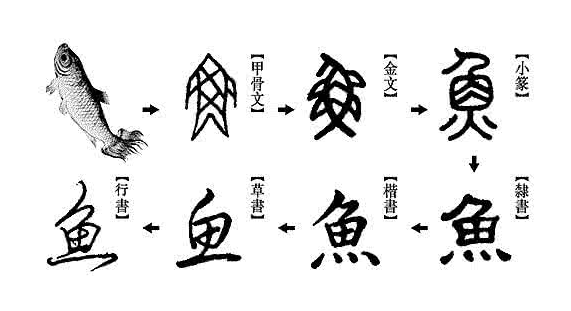
\includegraphics[scale=0.6]{picture/char.png}
    \caption{鱼字的演化过程}
    \label{char_fish}
\end{figure}

部首是构建合体字的主要单元。这一概念最早由公元2世纪汉朝的许慎提出,
他在其著作《说文解字》中将合体字中重复出现的部分加以归类,分成540个“部”。
“部”之后发展为现在的部首,
现在通用的部首由清朝康熙五十五年(1716年)成书的《康熙字典》所制定,共214个。

汉字的部首通常由某一个独体字演化而来,而且与英语等字母语言不同的是,
部首是汉字语义的重要组成部分。很多时候,
部首能够让我们在没有任何上下文的情况下大致理解或推测一个汉字的意义。
这也就是说,在学习汉字语义表示的时候,部首所固有的语义特征能够提供额外的信息。
举例来说,通过由“人”字演变而来的部首“亻”,我们可以很清楚的知道“你”、“他”、“伙”、
“侣”、“们”等字全部都和人有关。并且这种根据部首获得的语义信息与N-gram模型这类基于相邻$N$
个单词获得的信息本质上是不同的。因此在词向量模型中添加部首的语义特征能够
给每个词语增加丰富的语义信息,提升中文词向量的质量。

偏旁是构建合体字的另外一个重要单元。虽然在合体字特别是形声字中,
偏旁往往表示事物的读音,但是对于会意字与部分形式字,偏旁任然含有可利用的语义信息。
比如汉字“武”,它的部首为“止”,是“趾”的本字,表示脚,偏旁为“戈”,表示武器,
整体表示人拿着武器行走;对于汉字“茱”,部首的“艹”表示植物,偏旁“朱”则表示红色,兼
表示字音。所以只要善加利用,偏旁也能够为词向量的构建提供很多语义特征。

\section{中文文本表示方法}
\label{word_vec_model}
中文文本的词向量构建方法一直是中文自然语言处理领域的焦点。
在研究初期,研究者们尝试直接使用英文词向量工具
(如\ref{sect_word2vec}中介绍的CBOW模型和Skip-gram模型)
在经过分词之后的中文语料上训练词向量。
但是这种做法很明显存在问题:大多数英文词向量工具在训练时都将词作为最小的操作单位,
而忽略了词语内在的一些形态信息(morphological information)。和英语等字母文字不同,
中文词语之中的汉字任然含有丰富的语义信息。比如“智能”这个词,
它的语义信息一方面我们可以从语料中相关的上下文学习,就像word2vec模型一样。
另一方面我们也可以根据组成这个词的两个汉字“智”和“能”推测出来(“智”为智慧,“能”为能力)。

为了解决上述问题,充分利用中文词语的语义信息,陈志勇等人\citing{chen2015joint}在
普通CBOW模型上加入汉字信息,提出了CWE模型。随后Xu等人\citing{xu2016improve}在
CWE模型的基础上,赋予词中每个字权重,优化整个词向量模型。
但这些模型都没有利用汉字中的偏旁部首,忽略了所有文字内部的信息。

另一方面,Sun等人\citing{sun2014radical}在CBOW模型的基础上增加了部首信息来训练中文字向量;
Yu等人\citing{yu2017joint}在CWE模型中结合“部首-汉字”与“汉字-词”的信息,
设计了一个多粒度的词向量模型。但这些方法都只是简单的在模型中添加了部首信息,没有考虑
到部首的演化,即没有将部首与意义对应的汉字联系起来(比如“氵”-“水”),
这使得模型从部首获得的信息非常有限,影响生成的词向量的质量。


\section{部首信息增强的中文词向量构建方法}
根据上一小节中介绍的其他学者在中文词向量模型上的种种成果以及汉字中偏旁部首的特性,
本文设计了一种新的中文词向量模型——部首信息增强的中文词向量模型(Radical Enhanced Chinese Word Embedding,RECWE)。
RECWE以word2vec工具的CBOW模型为基础,在模型的预测层中增加一个代表“偏旁部首-汉字”信息的隐藏层,
增强每个词的语义信息。同时,RECWE将输入文本从简体转换为繁体,并对每个字的部首进行语义转换,
最大程度上丰富输入词语的语义信息。
\subsection{文本预处理}
由于实验所用的语料大多来自于互联网,其格式编码往往没有统一,所以需要首先进行相关处理,得到
一个相对整齐一致的文本数据。同时为了让词向量模型能够获取部首信息,还需要进行语义相关的一些
处理。整体的预处理流程包括:

(1)特殊字符过滤

网络搜集的数据常常是用户随意产生的非规范文本,里面会包含大量和文本语义无关的特殊字符与
标点符号,因此需要对这些符号进行过滤,只保留文本以及相关英文专有名词。

(2)全半角转换

由于使用的语料来源广泛,相互之间没有共同的格式规范,文本中的数字、英文字母等同时存在全角
和半角的格式,为了让之后的分词工作能够准确快速,需要将所有数字及字母统一转换为半角字符。

(3)分词

本文所使用的分词工具为java语言实现的Ansj中文分词开源库。该库基于n-Gram、CRF与HMM
算法,分词速度达到每秒钟大约200万字左右,准确率能达到96\%以上,并且实现了
中文分词、中文姓名识别、用户自定义词典、关键字提取、自动摘要、关键字标记等重要功能,
对于短文本语料有较好的表现。

(3)繁简转换

新中国成立后进行了一系列汉字简化工作,现阶段中国大陆地区使用的简体汉字是1956年发布的\citing{su2007hanzi}。
但在汉字简化工作中,存在一些不适当的简化,使得简化字的部首与原始繁体字的部首不同,
出现汉字语义上的偏差。例如繁体字中的“羆”字,分解后的偏旁部首为“罒”和“熊”,
意指一种很大的熊,可是简化后却变为了“罴”,相应的偏旁部首为“罢”和“灬”,失去了原来的含义。
而且简化工作还将多个繁体字归并为一个简体字,即“一简对多繁”,这就造成了理解上的困难和歧义,并生成了一批多音字,让简体词语中的字不能
很好的反应这个词的语义,增加了词向量模型学习词语语义的难度。比如繁体的词语“干(gān)涉”、“乾(gān)燥”、“幹(gàn)部”中的“干”、“乾”和“幹”,简化后统一变为
“干”字,让模型很难区分。

因此,为了更好的表达原始语料中文本的语义,让模型能够正确捕获中文词语中的部首的语义信息,
需要将原本的简体文本全部转换为繁体文本。本文使用汉语言处理包HanLP作为繁简转换工具,
该处理包能够有效区分同一个简体字对应的多个繁体字,并且可以识别简繁分歧词,
如“打印机”与“印表機”。

%(4)部首提取与语义转换

\subsection{部首信息增强的中文词向量模型}
\label{recwe_section}
本文提出的RECWE模型结合了中文的单词、汉字以及偏旁部首的语义信息,旨在构建适合中文的高效词向量。
RECWE模型基于CBOW模型\citing{mikolov2013distributed},
通过词的平均上下文向量和字与部首的平均上下文向量预测目标词,
并且使用这两个上下文向量的预测损失的和作为目标函数。
\begin{table}[h]
    \caption{常见部首转换表}
    \begin{tabular}{|c|c|c|c|}
        \hline
        部首 & 对应汉字 & 部首 & 对应汉字 \\
        \hline
        艹 & 艸 & 亻 & 人\\
        \hline
        刂 & 刀 & 犭 & 犬\\
        \hline
        灬 & 火 & 釒 & 金\\
        \hline
        麥 & 麥 & 飠 & 食\\
        \hline
        礻 & 示 & 月 & 肉\\
        \hline
        攵 & 攴 & 罒 & 网\\
        \hline
        扌 & 手 & 氵 & 水\\
        \hline
        糹 & 糸 & 耂 & 老\\
        \hline
        牜 & 牛 & 忄 & 心\\
        \hline
        衤 & 衣 & 王 & 玉\\
        \hline
        辶 & 走 & 疒 & 病\\
        \hline
    \end{tabular}
    \label{char_tran_form}
    \end{table}

为了让RECWE模型能够直接获取汉字的部首信息,训练时会将词语中的汉字拆解为
对应的偏旁部首。但是,根据\ref{radical_information}节中关于部首的介绍,
由某一个独体字演化而来的部首,
在合体字中会为了书写美观往往需要进行一定的拉伸或收缩,
来适应合体字整体的字型。例如“水”字在合体字中拉伸成了部首“氵”,
“食”字在合体中收缩为了部首“飠”,
仅仅使用“氵”来表示部首并不能显示出其本身蕴含的“水”的语义信息。
因此本文提取了常见字的部首并构建了一个转换表(如表\ref{char_tran_form}所示),
将部首转换为对应的独体字,从而让RECWE模型能够有效识别出这种内在联系,
比如“木”字与“案”、“板”、“森”、“李”等字,“水”字与“泉”、“河”、“海”等字。

RECWE模型结构如图\ref{RECWE}所示,其中$w_i$表示需要预测的目标词,$w_{i-1}$和$w_{i+1}$
分别表示文本中目标词$w_i$左边和右边的词。$c_{i-1}$和$c_{i+1}$表示$w_{i-1}$和$w_{i+1}$中的汉字,
$r_{i-1}$和$r_{i+1}$则分别表示$c_{i-1}$和$c_{i+1}$对应的部首(经过表\ref{char_tran_form}转换),
$s_{i-1}$和$s_{i+1}$表示$c_{i-1}$和$c_{i+1}$的偏旁。
以短句“江河流入大海”为例,RECWE模型在预测词语“流入”时,
输入的词向量序列$W$为$\{w_{i-1}(\mbox{江河}),w_{i+1}(\mbox{大海})\}$,
对应的汉字序列$C$为$\{c_{i-1}(\mbox{江},\mbox{河}),c_{i+1}(\mbox{大},\mbox{海})\}$,
部首序列$R$为$\{r_{i-1}(\mbox{水},\mbox{水}),r_{i+1}(\mbox{大},\mbox{水})\}$,
偏旁序列$S$为$\{s_{i-1}(\mbox{工},\mbox{可}),s_{i+1}(\mbox{大},\mbox{每})\}$。

RECWE模型通过在预测层将两个上下文向量并列以及共享隐藏层参数,字向量与偏旁部首向量在训练时能够很好的
影响词向量,从而让最终训练得到的词向量能够充分反映出词语内部汉字与部首的语义信息。
\begin{figure}[h]
    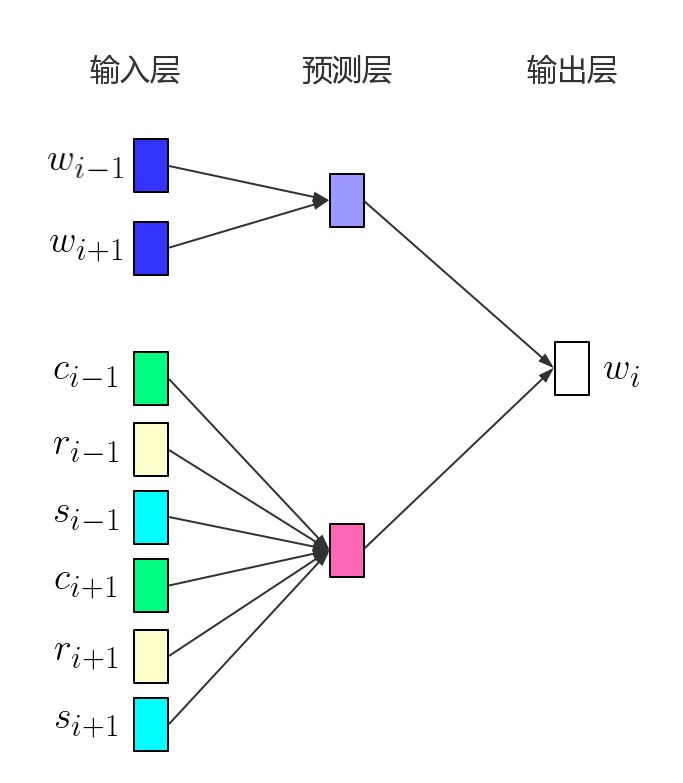
\includegraphics[scale=0.4]{picture/RECWE.png}
    \caption{RECEW模型结构}
    \label{RECWE}
\end{figure}

与CBOW模型类似的,RECWE模型的目标函数是两个上下文向量对于目标词$w_i$的条件概率的对数似然函数,
如公式\ref{RECWE_target_fun}所示。
\begin{equation}
    L\left ( w_i \right )= \sum_{k}^{2}\log P\left ( w_i | h_{i_k} \right )
    \label{RECWE_target_fun}
\end{equation}
其中$h_{i_1}$和$h_{i_2}$分别表示词的上下文向量和字与部首的上下文向量。
通过这样

每个上下文向量对于目标词$w_i$的条件概率$p\left( w_i|h_{i_k}\right )$可以利用softmax函数求解,
如公式\ref{conditional_pro_fun}所示。
\begin{equation}
    p\left ( w_i | h_{i_k} \right )=\frac{\exp \left ( h_{i_k}^{T}\hat{v}_{w_i} \right )}{\sum_{j=1}^{N}\exp \left ( h_{i_k}^{T}\hat{v}_{w_j} \right )},k=1,2
    \label{conditional_pro_fun}
\end{equation}
其中$\hat{v}_{w_i}$表示目标词$w_i$的“输出”向量,$\hat{v}_{w_j}$表示输入语料中每个词的“输出”向量,
$N$表示输入语料的长度。

上下文向量$h_{i_1}$是上下文窗口中每个词的“输入”向量的平均值,通过式\ref{word_context_fun}得到:
\begin{equation}
    h_{i_1}=\frac{1}{2T}\sum_{-T\leq j\leq T,j\neq 0}v_{w_{i+j}}
    \label{word_context_fun}
\end{equation}
式中的$T$表示上下文窗口的大小,$v_{w_{i+j}}$是上下文窗口中单词的“输入”向量。

类似的,字与部首的上下文向量$h_{i_2}$是上下文窗口中每个词对应的字及其偏旁部首的“输入”向量的平均值,计算公式如\ref{char_context_fun}所示。
\begin{equation}
    h_{i_2}=\frac{1}{X}\sum_{-T\leq j\leq T,j\neq 0} v_{c_{i+j}}+v_{r_{i+j}}
    \label{char_context_fun}
\end{equation}
其中$v_{c_{i+j}}$和$v_{r_{i+j}}$分别表示字和偏旁部首的“输入”向量,$X$为
$v_{c_{i+j}}$和$v_{r_{i+j}}$的数量。

于是,对于语料库$D$,RECWE模型的整体对数似然函数如公式\ref{overall_target_fun}所示。
\begin{equation}
    L\left ( D \right )=\sum_{w_i \in D}L\left ( w_i \right )
    \label{overall_target_fun}
\end{equation}

RECWE模型的训练算法采用CBOW模型实现的负采样(Negative Sampling,NEG)算法\citing{mikolov2013distributed},
该算法是NCE(Noise Contrastive Estimation,NCE)算法的一个简化版本,
其中心思想是将当前窗口内的词语分为正样本(需要预测的目标词)及负样本(目标词之外的其他词),
然后加权随机选取负样本进行更新,每个负样本的权重与其在语料库中出现的次数成正比,
以此来提高模型的训练速度并改善所得词向量的质量。
结合随机梯度上升技术,
基于负采样的RECWE模型能够快速获得中文词向量。



%添加点
%可以添加负采样的介绍

\section{部首信息增强的中文字向量构建方法}
%\subsection{中文字向量概述}
中文分词技术虽然已相对成熟,但准确率仍然达不到100\%,分词结果依然存在一定的错误。
特别是对于本文主要研究的中文短文本,由于其大多来自于用户在互联网中的互动,如腾讯空间说说、新浪微博、
淘宝商品评价等,相比于长文本具有很强的随意性,充斥着大量的口语化表达方式,
有些句子甚至存在语病,这更进一步增加了分词的难度,使得分词结果很不理想。
而错误的分词结果会极大影响后续的词向量模型,降低词向量的质量。

字向量是解决分词问题的一个方向,
来源于英文文本处理中字符级别(Character-level)的文本表示方式
\citing{zhang2015character}。
国内学者通过给汉字编码\citing{chen2015joint, 胡浩2017汉字固有属性},或将汉字转换为汉语拼音\citing{zhang2015character},
将文本表示为连续的向量,从而绕过分词的步骤,然后通过循环神经网络等深度学习技术直接从
字向量中学习文本特征,取得了不错的成果。但这些方法得到字向量类似于One-hot向量,
没有反应出每个字之间语义上的联系,忽略了大量的语义信息。
因此,作为RECWE词向量模型的补充,本文设计了一个能够利用汉字部首信息的字向量模型——部首信息增强的中文字向量模型(Radical Enhanced Chinese Character Embedding,RECCE),
为后续的分类模型提供更多的文本信息。

%\subsection{部首信息增强的中文字向量模型}
RECCE模型是RECWE模型的一个变形,它替换了输入层的词向量,
将模型的主要训练对象转换为字向量,网络结构图如图\ref{RECCE}所示,
其中$c_i$表示当前需要预测的目标字,其他符号与图\ref{RECWE}相同。
\begin{figure}
    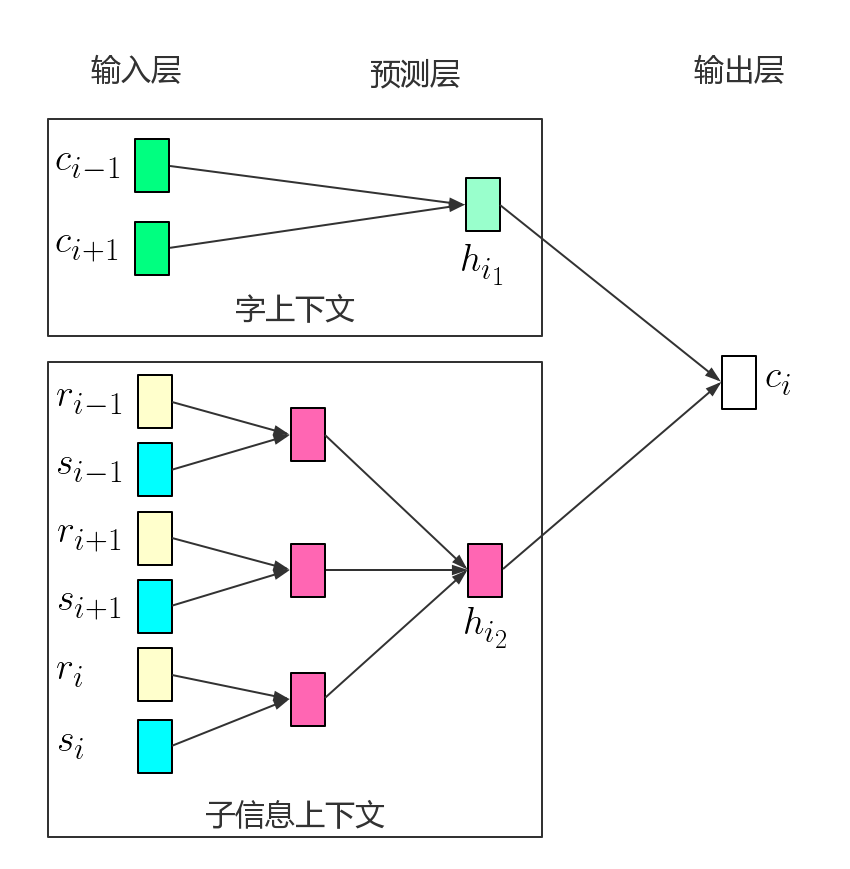
\includegraphics[scale=0.4]{picture/RECCE.png}
    \caption{RECCW模型结构}
    \label{RECCE}
\end{figure}

通过部首转换,RECCE模型将汉字映射到连续的向量空间,
克服了One-hot类型的字向量的种种问题,
让具有相同语义的字向量能够在空间上彼此靠近(如“病”、“疤”、“癌”等字)
,增强了字向量对于文本的表现力。
同时对于某些非常短小的文本,如新闻标题、微信聊天记录等,
使用词向量进行表示得到的数据长度往往不超过10,还可能存在分词错误,不利于后续分类模型的特征提取工作。
使用字向量则一定程度上丰富了文本的信息量,让分类模型能够获取到更多的特征,
避免分词错误带来的影响,提升分类准确率。

\section{实验及其结果分析}
为了验证算法获得的词向量与字向量的可行性与有效性,本节将根据来源于“今日头条”新闻网的新闻标题数据进行实验。
实验实现前面介绍的RECWE模型与RECCE模型,同时实现了\ref{word_vec_model}小节中提到的word2vec工具、
CWE模型\citing{chen2015joint}、
SCWE模型\citing{xu2016improve}、
JWE模型\citing{yu2017joint}与\ref{research_status}小节中提到的charCBOW模型\citing{li2015component}用于对比实验。
词向量、字向量的有很多种评价方法,本实验主要使用词相似度(Word Similarity)与词类比(Word Analogy)方法
来评价不同模型训练出的词向量,使用字相似度(Character Similarity)方法来评价不同模型训练出的字向量。
\subsection{部首信息增强的中文词向量模型实验对比}
训练语料使用RECWE模型使用的Ansj工具分词,哈工大以及百度停用词表过滤掉新闻中的停用词,
所有词向量模型采用统一的训练参数,具体如表\ref{word_vec_arg_form}所示。
\begin{table}[h]
    \caption{词向量训练参数表}
    \begin{tabular}{|c|c|c|}
        \hline
        参数名 & 参数意义 & 参数值 \\
        \hline
        size & 词向量纬度 & 200 \\
        \hline
        alpha & 学习速率 & 0.025 \\
        \hline
        mincount & 语料中低频词的出现词频 & 5 \\
        \hline
        sample & 高频词汇的随机降采样的配置阈值 & 1e-4 \\
        \hline
        workers & 训练的并行数 & 4 \\
        \hline
        iter & 迭代次数 & 5 \\
        \hline
        window & 当前词与预测词的最大距离 & 5 \\
        \hline
    \end{tabular}
    \label{word_vec_arg_form}
    \end{table}

(1)词相似度

词相似度主要用来评估词向量判断语义相近的单词对的能力\citing{yu2017joint}。
本实验选择了文献\cite{chen2015joint}提供的两个不同的相似词数据库wordsim-240和wrodsim-296,
它们分别包含240个中文单词对与296个中文单词对,每个单词对都包含一个人工标注的相似度。
wordsim-240主要针对语义上有联系的单词,wordsim-296则针对同义词,
部分数据如表\ref{wordsim-240_form}与表\ref{wordsim-296_form}所示。

\begin{table}[h]
    \caption{wordsim-240数据节选}
    \begin{tabular}{|c|c|c|}
        \hline
        单词1 & 单词2 & 相似度 \\
        \hline
        李白 & 诗 & 9.2 \\
        \hline
        浏览器 & 网页 & 8.95 \\
        \hline
        医生 & 职责 & 8.85 \\
        \hline
        白天 & 晚上 & 8.8 \\
        \hline
        学生 & 学校 & 8.71 \\
        \hline
        法官 & 法律 & 8.65 \\
        \hline
        员工 & 公司 & 8.65 \\
        \hline
        ... & ... & ... \\
        \hline
        教授 & 黄瓜 & 0.5 \\
        \hline
        鸟 & 自行车 & 0.5 \\
        \hline
        蛋白质 & 文物 & 0.15 \\
        \hline
    \end{tabular}
    \label{wordsim-240_form}
    \end{table}

\begin{table}[h]
\caption{wordsim-296数据节选}
\begin{tabular}{|c|c|c|}
    \hline
    单词1 & 单词2 & 相似度 \\
    \hline
    足球 & 足球 & 4.98 \\
    \hline
    老虎 & 老虎 & 4.8888888889 \\
    \hline
    恒星 & 恒星 & 4.7222222222 \\
    \hline
    入场券 & 门票 & 4.5962962963 \\
    \hline
    ... & ... & ... \\
    \hline
    签名 & 暂停 & 0.304 \\
    \hline
    股票 & 美洲豹 & 0.304 \\
    \hline
    延迟 & 种族主义 & 0.262962963 \\
    \hline
\end{tabular}
\label{wordsim-296_form}
\end{table}

对于每个词向量模型,单词对的相似度通过这两个单词相应的词向量的余弦距离来表示。
实验最后依靠计算词向量得到的相似度与相似词数据库中人工标注的相似度之间的spearman相关系数(Spearman Correlation)\citing{mikolov2013distributed}
判断词向量的好坏,spearman相关系数越高,代表该词向量越能体现单词之间的相关性。
具体的实验结果如表\ref{word_vec_result}所示。
\begin{table}[ht]
    \caption{词向量评估结果}
    \begin{tabular}{|c|c|c|}
        \hline
        模型 & wordsim-240 & wordsim-296 \\
        \hline
        word2vec & 0.4221 & 0.4479 \\
        \hline
        CWE & 0.43635 & 0.4750 \\
        \hline
        SCWE & 0.4311 & 0.4648 \\
        \hline
        JWE & 0.4467 & 0.5831 \\
        \hline
        RECWE & 0.4962 & 0.5849 \\
        \hline
    \end{tabular}
    \label{word_vec_result}
    \end{table}

从结果中可以看出,在两个相似词库上,RECWE模型的表现都优于其他模型。
CWE模型和SCWE模型相比word2vec结果有所提升,但由于只利用了单词中的汉字信息,
所以相较于添加了部首信息的JWE模型与RECWE模型结果要差。还可以看到,在wordsim-240数据库
上,RECWE模型与JWE模型相比有较大提升。
这主要是因为该数据库中包含的大多是语义上有一定从属关系的单词对,而拥有部首转义机制的
RECWE模型能够很好的找到这样的关系。比如单词对“淋浴”与“水”,RECWE模型会在预处理阶段把
“淋”字和“浴”字的偏旁“氵”转义为“水”,然后在模型训练阶段就可以发现“淋浴”与“水”之间的内在联系。

(2)词类比

词类比是另一种衡量词向量好坏的技术,它主要判断词向量是否能够体现出单词对之间的语言规律\citing{mikolov2013linguistic}。
举例来说,给定单词关系组“北京-中国:东京-日本”,一个好的词向量就应该让单词“日本”的词向量$vec\left(\mbox{日本}\right)$
接近式子“$vec\left(\mbox{中国}\right)$-$vec\left(\mbox{北京}\right)$+$vec\left(\mbox{东京}\right)$”产生的向量。
也就是说,给定一个类比关系“$a$-$b$:$c$-$d$”,如果词向量能够通过公式\ref{word_analogy_eqn}在词表中寻找向量$x$来
使关系“$a$-$b$:$c$-$x$”成立,那么就判定这个词向量包含这个类比关系。
\begin{equation}
    \arg \max_{x\neq a,x\neq b,x\neq c}\cos \left ( \vec{b}-\vec{a}+\vec{c},\vec{x} \right )
    \label{word_analogy_eqn}
\end{equation}

本次实验使用文献\cite{chen2015joint}提供的中文词类比数据库,
包含了1124组词类比关系,每组类比关系包含4个单词,所有类比关系分为三个类别:
“首都”(677组)、“省会”(175组)、“人员”(272组)。具体数据如表\ref{word_analogy_table}所示。
\begin{table}[ht]
    \caption{词类比数据库(部分)}
    \begin{tabular}{|c|c|c|}
        \hline
        类别 & 单词对1 & 单词对2 \\
        \hline
        首都 & 曼谷-泰国 & 北京-中国 \\
        \hline
        首都 & 东京-日本 & 柏林-德国 \\
        \hline
        首都 & 伦敦-英国 & 开罗-埃及 \\
        \hline
        省会 & 长春-吉林 & 哈尔滨-黑龙江 \\
        \hline
        省会 & 南昌-江西 & 南京-江苏 \\
        \hline
        省会 & 广州-广东 & 成都-四川 \\
        \hline
        人员 & 爸爸-妈妈 & 兄弟-姐妹 \\
        \hline
        人员 & 国王-王后 &  父亲-母亲\\
        \hline
        人员 & 爷爷-奶奶 & 叔叔-阿姨 \\
        \hline
    \end{tabular}
    \label{word_analogy_table}
    \end{table}

实验用准确率作为结果指标,准确率越高,表明词向量包含的词类比关系越多,
三类词类比的实验结果如表\ref{word_analogy_resutl}所示,
总体结果见图\ref{word_analogy_all_resutl}所示。
\begin{table}[ht]
    \caption{各类类比关系实验结果}
    \begin{tabular}{|c|c|c|c|}
        \hline
        词向量模型 & 首都 & 省会 & 人员 \\
        \hline
        word2vec & 0.11816 & 0.11428 & 0.34558 \\
        \hline
        CWE & 0.20787 & 0.14285 & 0.32720 \\
        \hline
        SCWE & 0.21381 & 0.14022 & 0.33021 \\
        \hline
        JWE & 0.22101 & 0.16 & 0.32352 \\
        \hline
        RECWE & 0.23632 & 0.18285 & 0.38603 \\
        \hline
    \end{tabular}
    \label{word_analogy_resutl}
    \end{table}

\begin{figure}[!h]
    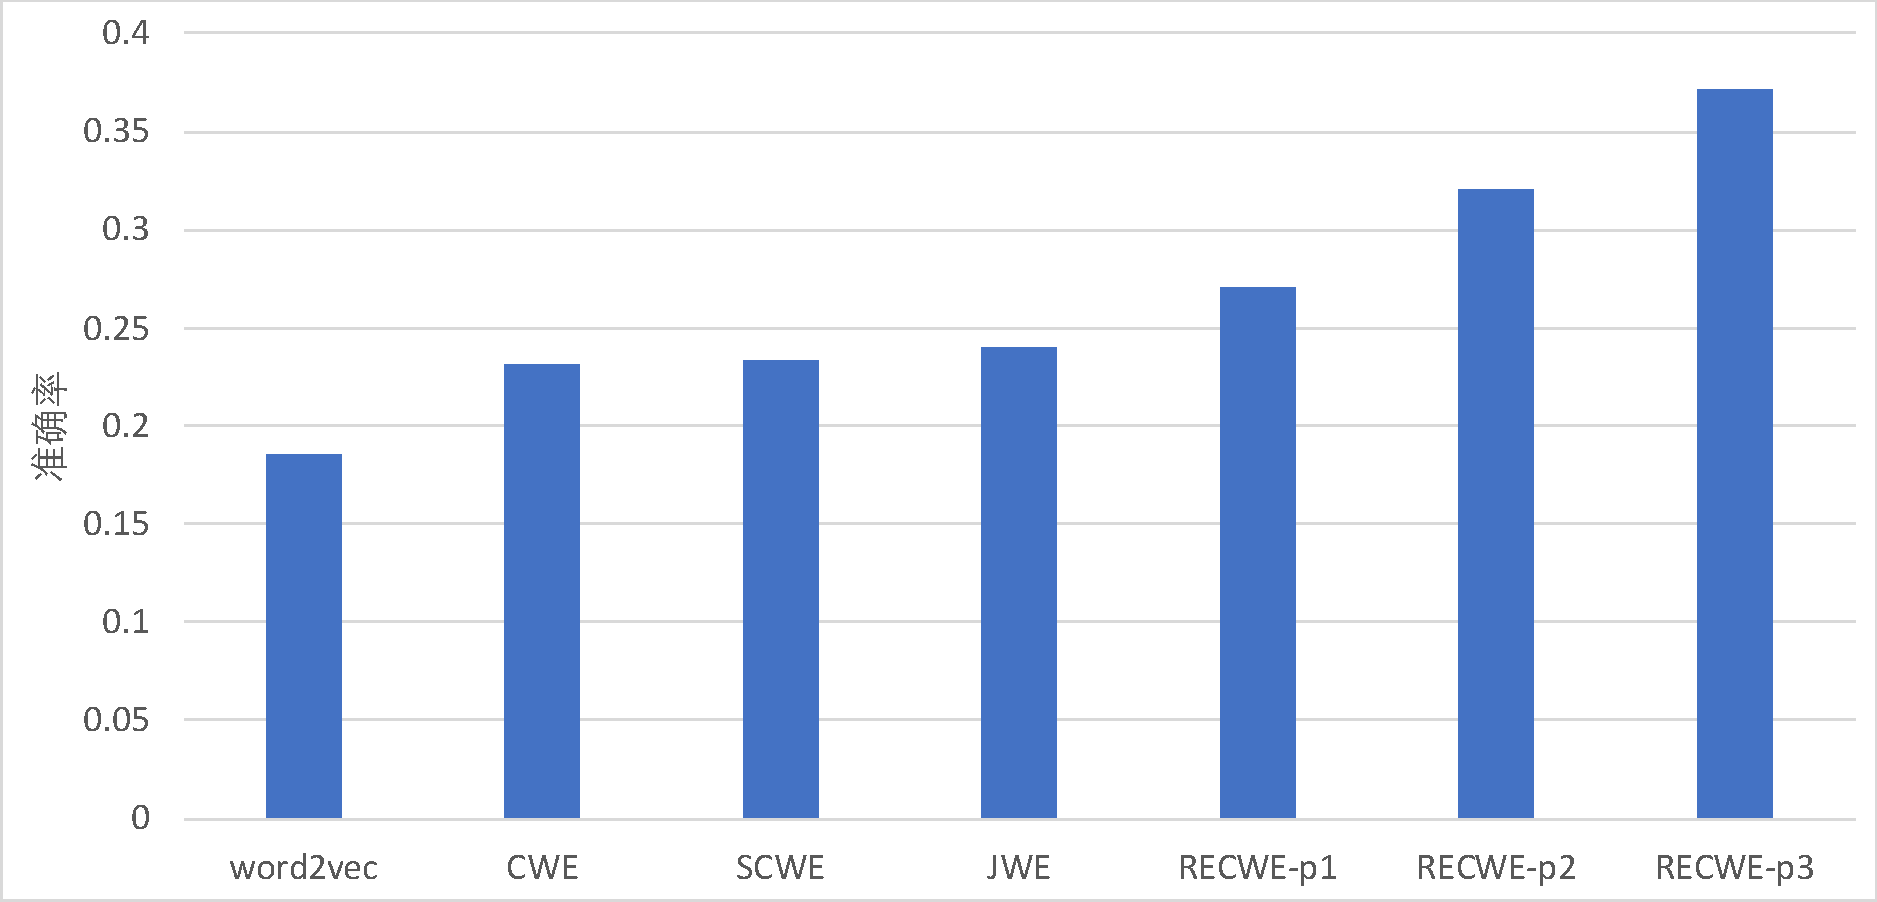
\includegraphics[scale=0.5]{picture/word_analogy_result.pdf}
    \caption{词类比整体实验结果}
    \label{word_analogy_all_resutl}
\end{figure}

从这两个结果中可以看出,同其他词向量模型相比,RECWE模型在三类类比关系上都取得了
最优的结果,表明部首信息能够增强模型在语言规律上的表现力。特别在“人员”类上,
部首转义机制让RECWE模型能够相对容易的根据
部首发现词对之间的关系,如通过部首“女”联系“妈妈”、“姐姐”等词,所以结果中相对JWE模型准确率有较大提升。而对于“首都”这类包含大量音译词的类别,
其内部部首不能提供额外语义,则提升较小。

\subsection{部首信息增强的中文字向量模型实验对比}
本实验通过字相似度技术比较不同模型训练得到的词向量,
使用的字相似度数据库类似上一个小节中使用的词相似度数据库,
描述了400个常见字的关联关系,部分数据如表\ref{charsim_form}所示。
\begin{table}[h]
    \caption{字相似度数据库(部分)}
    \begin{tabular}{|c|c|c|}
        \hline
        汉字1 & 汉字2 & 相似度 \\
        \hline
        犬 & 狗 & 11.425 \\
        \hline
        癌 & 病 & 10.525 \\
        \hline
        七 & 列 & 0.5 \\
        \hline
        车 & 鸟 & 0.427 \\
        \hline
    \end{tabular}
    \label{charsim_form}
    \end{table}
字向量模型的训练参数与上一小结中的训练参数相同,实验结果见表\ref{char_vec_result}所示。
\begin{table}[!h]
    \caption{字向量评估结果}
    \begin{tabular}{|c|c|}
        \hline
        模型 &  spearman相关系数\\
        \hline
        word2vec & 0.47693 \\
        \hline
        charCBOW & 0.48852 \\
        \hline
        JWE & 0.56075 \\
        \hline
        RECCE & 0.59409 \\
        \hline
    \end{tabular}
    \label{char_vec_result}
    \end{table}

可以看到,RECCE模型训练的字向量总体上有了一个较优秀的结果,表明添加部首的语义信息对于
字向量的训练同样有效。
\section{本章小结}
本章节主要介绍中文短文本的表示方法,首先分析了汉字的演变以及汉字部首对于汉字语义的贡献,
接着总结了近几年相关学者在中文文本表示上的一些研究,然后在此基础上提出了两种新的
文本表示模型——部首信息增强的词向量模型与部首信息增强的字向量模型,最后设计实验
与其他模型进行对比,实验结果表明模型能够有效提升词向量与字向量的质量,为后续
分类模型提供充实的基础。